\section{Imperfect Scaling Study}\label{sec:case-study}

\if 0
\begin{figure}[ht]
%Terrible hack
%note this may break if the graph ends up in the other column so if the graph is too far left, adjust this
\hspace{-2.5em}{
%The graph
\begin{tikzpicture}
  \begin{axis}[
      ylabel={\footnotesize Cycles per operation (normalized)},
      xlabel={\footnotesize Frequency (MHz)},
      legend pos=north west,
    ]
    \addplot table[y expr=\thisrowno0*\thisrowno1/(1200*3.00)] {./cache_misser_data.txt};
    \addlegendentry {Random};
    \addplot table[y expr=\thisrowno0*\thisrowno1/(1200*1.56)]  {./normal_data.txt};
    \addlegendentry {Sequential};
    
  \end{axis}
\end{tikzpicture}
}
\caption{Effect of Cache Misses}
\label{fig:cache}
\end{figure}
\fi 

\begin{figure}
  \begin{center}
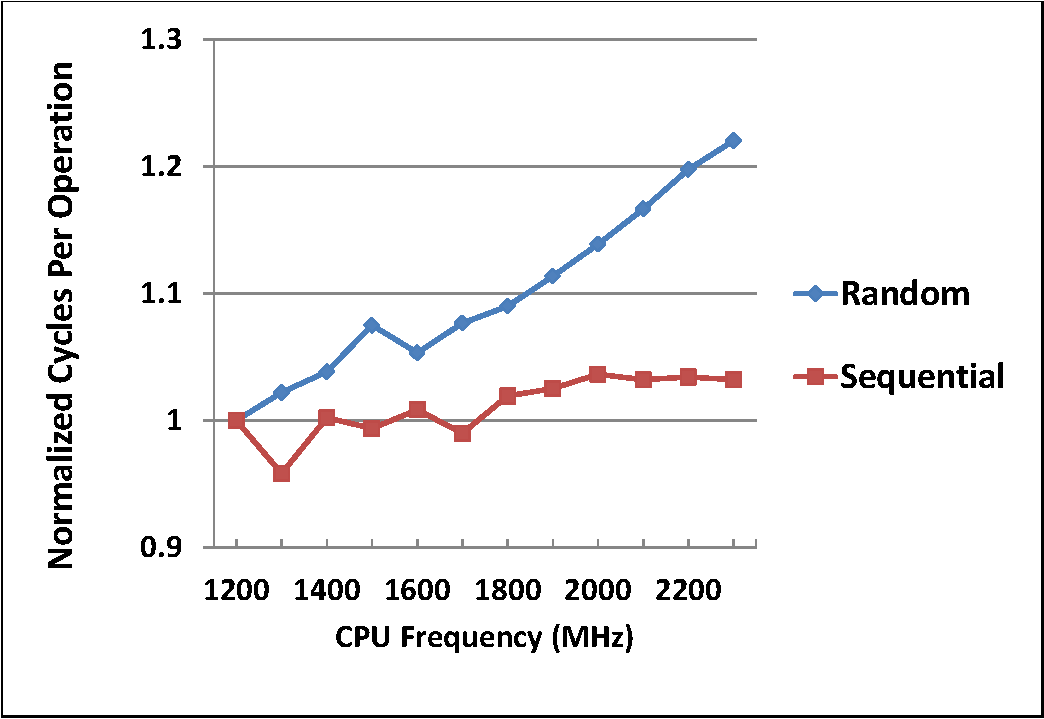
\includegraphics[width=\linewidth]{figs/case-crop.pdf}
  \end{center}
  \vspace{-0.1in}
  \caption{Effect of Cache Misses}
	\label{fig:case}
\end{figure}



An assumption often made, with respect to the power usage 
is that on a given CPU, changing the frequency will change the CPU performance by the corresponding amount.
However, this is only true when considering CPU execution, 
but there exist other pieces who's performance do not scale along with CPU frequency.
One example would be memory. CPU caches hide much of this latency, but cache misses can be particularly damaging to efficiency, since the time frame is too short for the operating system to handle them intelligently, or even be aware of them except retrospectively, yet they take long enough that they measurably decrease performance and or efficiency.
 
To demonstrate this effect, we wrote the following microbenchmark, where a process takes a large (32MB) array and copies a random entry to another random entry. Then we set the CPU to a variety of frequencies and measured execution time.  This was then compared to another process that did the same type of work, copying data from one point to another, but did so sequentially, thus avoiding most of the cache misses. As expected for both processes the time to execute decreases as CPU frequency increase, but more interestingly, we can also plot the efficiency, computed here as the time to execute times the frequency, which represents the number of clock cycles required to execute the process. For ease of comparison these were then normalized.

 Since both processes do the same amount of computation, the only factor that can affect performance and efficiency is the memory access pattern. And if performance scaled perfectly with CPU frequency, we would expect a nearly flat line, as we see in the case of sequential access. But with random accesses, we see instead that the cycles per instruction increase as the frequency increases, clearly demonstrating a decrease in efficiency, with the final result being that at 2300MHz, we are ~20\% less efficient than at 1200MHz

There are two mitigating factors with respect to this issue. First is programming practices, Since cache misses are a well known performance issue, many applications are already written to avoid them as much as reasonable. Second is the hardware. In particular modern processors have both hyperthreading and out of order execution, both of these features allow the processor to potentially work on other instructions which do not require the data being fetched. Nonetheless, as we will demonstrate, with some workloads, the inevitable constraint is memory bandwidth and/or latency, and in these cases a decrease in CPU frequency may very well lead to efficiency gains.



